% Provenance (never printed): see sources/outline_sources.md (Year 2: natural hazards and risks
% quantified --- recurrence, probabilistic hazard, slope stability, tsunamis, floods, warning).
% Terminology from the UN report A/71/644 (UNDRR); the 475-year convention from the USGS
% Earthquake Hazards 201 page; the ground-motion prediction equation of Boore, Joyner and Fumal
% (USGS Open-File Report 93-509); run-ups from the NOAA NCEI tsunami database; the 1999 Vargas
% debris flows from USGS Open-File Report 01-0144. Ledger rows in sources/ledger/book4.md;
% curves and numbers from figdata/bachelor-2/hazards.py and the Book 4 second-writer scratch
% calculator calc/ch28.py. Hazards are described and quantified physically only: no advice.
\chapter{Ameaças e riscos geológicos}\label{ch:b2:geological-hazards}

Um edifício projetado para o movimento do solo que é excedido, em média, uma vez em 475 anos tem
uma chance em dez de enfrentá-lo durante uma vida útil de cinquenta anos. As duas afirmações são o mesmo número
lido de duas maneiras, e passar de uma à outra é o trabalho diário da ciência das ameaças. Este capítulo
constrói suas ferramentas: a probabilidade dos eventos raros, a \omterm{def:b2:geological-hazards:psha}{curva de ameaça} de um local, a estabilidade de uma
encosta, a velocidade e a \omterm{def:b2:geological-hazards:tsunami}{altura máxima de inundação de um tsunami}, a frequência das cheias, e a física que fixa
quanto aviso prévio cada ameaça pode dar.
% ledger: usgs:eh201-475

\begin{recall}
\textbf{Dos volumes escolares}: ameaça natural, desastre natural e deslizamento; vulnerabilidade,
risco, prevenção e o mapa de ameaças; o tsunami; o \omterm{def:b2:geological-hazards:return}{período de retorno} de uma cheia, e a fórmula dos postos
$T = (n + 1)/m$ para um registro de $n$ picos anuais. \textbf{Do volume do primeiro ano}: a
lei de Gutenberg--Richter $\log_{10} N(\geq M) = a - bM$ e seu valor b; o momento sísmico e a magnitude
de momento; a pressão de fluido nos poros, a tensão efetiva $\sigma' = \sigma - u$ e o critério de ruptura
de Coulomb $\tau = c' + \sigma' \tan\varphi'$. \textbf{Do \cref{ch:b2:eruptive-styles}}: as \omterm{def:b2:eruptive-styles:pdc}{correntes de densidade
piroclásticas}, os \omterm{def:b2:eruptive-styles:lahar}{lahares} e a queda de \omterm{def:b2:eruptive-styles:tephra}{tefra}. \textbf{Dos livros de matemática}: as distribuições de Poisson e
exponencial, a distribuição normal e sua função de distribuição $\Phi$.
\textbf{Do volume do segundo ano dos livros de física}: a relação de dispersão das ondas de gravidade de superfície,
$\omega^2 = gk\tanh(kh)$.
\end{recall}

\section{Ameaça, exposição e risco}\label{sec:b2:geological-hazards:risk}

\begin{definition}[Ameaça geológica, exposição, risco de desastre]\label{def:b2:geological-hazards:risk}
Uma \emph{ameaça geológica}\index{ameaça geológica} é um processo ou fenômeno que se origina
nos processos internos da Terra --- um terremoto, uma erupção, um movimento de massa como um
deslizamento ou um \omterm{def:b2:geological-hazards:slope}{fluxo de detritos} --- e pode causar perda de vidas, ferimentos, danos ou perturbações. Ela é
caracterizada por sua localização, sua intensidade ou magnitude, e sua frequência ou probabilidade. A
\emph{exposição}\index{exposição (a uma ameaça)} a uma ameaça é a situação das pessoas, dos
edifícios, da infraestrutura e de outros bens situados onde a ameaça pode chegar, medida por seu
número ou seu valor. O \emph{risco de desastre}\index{risco de desastre} é a perda potencial de vidas,
de saúde ou de bens que poderia ocorrer num período dado, determinada probabilisticamente a partir da
ameaça, da exposição e da vulnerabilidade do que está exposto.
\end{definition}
% ledger: undrr:hazard, undrr:geological, undrr:exposure, undrr:disaster-risk, undrr:vulnerability

A terminologia internacional classifica os tsunamis à parte: desencadeados por terremotos e outros
eventos geológicos, eles se tornam um processo oceânico e atingem como uma ameaça costeira, ligada à água.
Este capítulo trata-os com as outras, porque sua fonte é geológica.
% ledger: undrr:geological

A definição contém um produto. Se eventos de intensidade $i$ ocorrem a uma taxa anual
$\lambda_i$, se os bens expostos valem $E$, e se um evento de intensidade $i$ destrói uma
fração $V_i$ deles (a vulnerabilidade, entre 0 e 1), a perda anual esperada é
\begin{equation}
L = \sum_i \lambda_i \, E \, V_i ,
\label{eq:b2:geological-hazards:loss}
\end{equation}
frequentemente abreviada como risco = ameaça $\times$ \omterm{def:b2:geological-hazards:risk}{exposição} $\times$ vulnerabilidade. O risco anula-se quando
qualquer fator se anula: um vulcão violento numa ilha vazia, uma cidade populosa num \omterm{def:b2:precambrian-earth:craton}{cráton} tranquilo, ou
edifícios que resistem ao abalo. A ciência das ameaças mede o primeiro fator; a figura abaixo
o situa entre os três.

\begin{omfigure}
\centering
\begin{tikzpicture}[font=\small]
\fill[omThm!14] (90:1.05) circle (1.55);
\fill[omDef!14] (210:1.05) circle (1.55);
\fill[black!8] (330:1.05) circle (1.55);
\begin{scope}
\clip (90:1.05) circle (1.55);
\clip (210:1.05) circle (1.55);
\fill[omThm!45!omDef!45] (330:1.05) circle (1.55);
\end{scope}
\draw[omThm, thick] (90:1.05) circle (1.55);
\draw[omDef, thick] (210:1.05) circle (1.55);
\draw[black!60, thick] (330:1.05) circle (1.55);
\node[align=center, anchor=south] at (0,2.65) {\textbf{ameaça} {\scriptsize (taxa $\lambda_i$, intensidade)}};
\node[align=right, anchor=east] at (-2.55,-1.35) {\textbf{exposição}\\[-1pt]{\scriptsize bens $E$}};
\node[align=left, anchor=west] at (2.55,-1.35) {\textbf{vulnerabilidade}\\[-1pt]{\scriptsize fração perdida $V_i$}};
\node[align=center, font=\scriptsize\bfseries] at (0,0) {risco};
\end{tikzpicture}
\par\smallskip{\small Os três fatores do \omterm{def:b2:geological-hazards:risk}{risco de desastre}. A perda esperada só é não nula onde
os três se sobrepõem: uma ameaça que atinge algo exposto e capaz de ser prejudicado.}
\end{omfigure}

\section{A probabilidade dos eventos raros}\label{sec:b2:geological-hazards:probability}

\begin{definition}[Período de retorno]\label{def:b2:geological-hazards:return}
Sejam eventos de um tipo dado --- uma cheia acima de uma vazão, um movimento do solo acima de um nível, um
terremoto acima de uma magnitude --- que ocorrem a uma taxa anual média $\lambda$. Seu \emph{período de
retorno}\index{período de retorno} é $T = 1/\lambda$: o intervalo médio entre dois deles, e o
inverso de sua taxa anual, não um calendário.
\end{definition}
% ledger: usgs:eh201-475

\begin{definition}[Probabilidade de excedência]\label{def:b2:geological-hazards:poisson}
A \emph{probabilidade de excedência}\index{probabilidade de excedência} de um nível num tempo de exposição $t$
é a probabilidade de que o nível seja igualado ou excedido pelo menos uma vez durante $t$.
\end{definition}

\begin{proposition}[Modelo de recorrência de Poisson]\label{prop:b2:geological-hazards:poisson}
Suponha-se que os eventos ocorram um de cada vez\index{modelo de recorrência de Poisson}, independentemente uns
dos outros e do tempo decorrido, a uma taxa média constante $\lambda = 1/T$. Então o número $N$ de
eventos num tempo $t$ segue a distribuição de Poisson de média $\lambda t$; a \omterm{def:b2:geological-hazards:poisson}{probabilidade de excedência}
em $t$ é
\begin{equation}
P(t) = 1 - e^{-t/T};
\label{eq:b2:geological-hazards:poisson}
\end{equation}
e o intervalo entre eventos sucessivos segue a distribuição exponencial de média $T$.
\end{proposition}

\begin{proof}
Seja $P_k(t)$ a probabilidade de $k$ eventos em $[0, t]$. Num intervalo curto $\mathrm{d}t$ um
evento ocorre com probabilidade $\lambda\,\mathrm{d}t$, independentemente do passado, e dois com uma
probabilidade de ordem superior. Logo $P_0(t + \mathrm{d}t) = P_0(t)(1 - \lambda\,\mathrm{d}t)$, isto é,
$P_0' = -\lambda P_0$ com $P_0(0) = 1$: $P_0(t) = e^{-\lambda t}$, e $P(t) = 1 - P_0(t)$. Da
mesma forma $P_k' = \lambda(P_{k-1} - P_k)$ para $k \geq 1$, resolvido por indução:
$P_k(t) = (\lambda t)^k e^{-\lambda t}/k!$, a distribuição de Poisson de média $\lambda t$. A partir de
um evento, o mesmo argumento dá a probabilidade de que o seguinte venha depois de $t$:
$e^{-\lambda t}$, a função de sobrevivência da distribuição exponencial, cuja média é
$\int_0^\infty e^{-\lambda t}\,\mathrm{d}t = 1/\lambda = T$.
\end{proof}

Duas consequências são usadas em toda parte. Para uma probabilidade $p$ num tempo de exposição $t$, o \omterm{def:b2:geological-hazards:return}{período
de retorno} é $T = -t/\ln(1 - p)$: \qty{10}{\percent} em 50 anos dá $T = 50/0.10536 =
474.6$ anos, o movimento ``de 475 anos'' das normas de construção, e \qty{2}{\percent} em 50 anos
dá 2475 anos. E quando $t \ll T$, $P \approx t/T$: a taxa pode ser lida como uma
probabilidade por ano. Ao longo de um \omterm{def:b2:geological-hazards:return}{período de retorno} inteiro, ao contrário, a probabilidade é $1 - e^{-1} =
\qty{63}{\percent}$, não 1. A figura abaixo (à esquerda) traça \eqref{eq:b2:geological-hazards:poisson}
para três \omterm{def:b2:geological-hazards:return}{períodos de retorno}.
% ledger: usgs:eh201-475
% values: T 474.561 and 2474.92 years; P(50|475) 0.0999 (hazards.py numbers)

O modelo é verdadeiro? O catálogo global de terremotos de magnitude pelo menos 7 contém 696 eventos
de 1976 a 2025, 695 intervalos com uma média de 26.2 dias. Se fossem um processo de Poisson,
a fração de intervalos mais longos que $t$ seria $e^{-t/26.2}$, uma reta num eixo
logarítmico. A figura abaixo (à direita) mostra que quase é: \qty{30.4}{\percent} dos intervalos são
mais longos que 30 dias, contra \qty{31.8}{\percent} para o modelo, e o desvio-padrão dos
intervalos é 1.07 vez sua média, contra exatamente 1. O defeito está nos intervalos curtos: 36 pares
caem no mesmo dia, réplicas e dupletos que um processo sem memória não agruparia. Os mapas de
ameaça por isso removem de um catálogo os eventos dependentes, desagrupando-o, de modo que os
choques principais restantes possam ser tratados como um processo de Poisson; suas taxas por magnitude vêm da
lei de Gutenberg--Richter.
% ledger: data:usgs-comcat, usgs:eh201-poisson
% values: m7_events 696, mean 26.2245 d, cv 1.06891, same-day 36, frac>30 d 0.303597 vs 0.318552

\begin{omfigure}
\centering
\begin{minipage}[b]{0.49\linewidth}\centering
\begin{tikzpicture}
\begin{axis}[omrecord, width=0.96\linewidth, height=5.2cm, xmin=0, xmax=200, ymin=0, ymax=1,
  xlabel={tempo de exposição $t$ (anos)}, ylabel={probabilidade de excedência},
  tick label style={font=\scriptsize}, label style={font=\small},
  xtick={0,50,100,150,200}, ytick={0,0.2,...,1}]
% computed in figdata/bachelor-2/hazards.py part poisson
\addplot[omThm, line width=1pt] table[x=t_yr, y=P50] {figdata/out/bachelor-2-hazards-poisson.dat};
\addplot[omDef, line width=1pt] table[x=t_yr, y=P475] {figdata/out/bachelor-2-hazards-poisson.dat};
\addplot[black!70, line width=1pt, densely dashed] table[x=t_yr, y=P2475] {figdata/out/bachelor-2-hazards-poisson.dat};
\draw[black!50, densely dotted] (axis cs:50,0) -- (axis cs:50,1);
\fill[omDef] (axis cs:50,0.1) circle (1.8pt);
\node[font=\scriptsize, text=omThm, anchor=west] at (axis cs:62,0.86) {$T = 50$};
\node[font=\scriptsize, text=omDef, anchor=west] at (axis cs:120,0.34) {$T = 475$};
\node[font=\scriptsize, text=black!70, anchor=west] at (axis cs:120,0.12) {$T = 2475$};
\node[font=\scriptsize, anchor=west, text=omDef] at (axis cs:52,0.2) {\qty{10}{\percent}};
\end{axis}
\end{tikzpicture}
\end{minipage}\hfill
\begin{minipage}[b]{0.49\linewidth}\centering
\begin{tikzpicture}
\begin{axis}[omrecord, width=0.93\linewidth, height=5.2cm, xmin=0, xmax=120, ymode=log,
  ymin=0.008, ymax=1.1, xlabel={intervalo $t$ (dias)}, ylabel={fração de intervalos $> t$},
  tick label style={font=\scriptsize}, label style={font=\small}, xtick={0,30,60,90,120},
  legend style={at={(0.03,0.03)}, anchor=south west, font=\scriptsize, draw=black!30},
  legend cell align=left]
% computed in figdata/bachelor-2/hazards.py part survival; ledger: data:usgs-comcat
\addplot[omThm, only marks, mark=*, mark size=1.2pt] table[x=t_day, y=observed] {figdata/out/bachelor-2-hazards-survival.dat};
\addlegendentry{$M \geq 7$, de 1976 a 2025}
\addplot[black, line width=0.9pt] table[x=t_day, y=poisson] {figdata/out/bachelor-2-hazards-survival.dat};
\addlegendentry{Poisson, média de 26.2 dias}
\end{axis}
\end{tikzpicture}
\end{minipage}
\par\smallskip{\small À esquerda: a probabilidade de pelo menos um evento num tempo de exposição $t$ para
\omterm{def:b2:geological-hazards:return}{períodos de retorno} de 50, 475 e 2475 anos; o evento de 475 anos tem uma chance de \qty{10}{\percent} em 50
anos. À direita: os intervalos entre os 696 terremotos de magnitude pelo menos 7 do catálogo
global de 1976--2025, comparados com a lei exponencial de um processo de Poisson de mesma taxa. Dados:
catálogo ANSS ComCat do USGS.}
\end{omfigure}

\section{A ameaça sísmica}\label{sec:b2:geological-hazards:seismic}

\begin{definition}[Análise probabilística da ameaça sísmica, equação de predição do movimento do solo, aceleração de pico do solo, curva de ameaça]\label{def:b2:geological-hazards:psha}
A \emph{aceleração de pico do solo}\index{aceleração de pico do solo} (PGA) num local é a maior
aceleração horizontal absoluta do solo durante um terremoto, expressa em geral como uma
fração de $g$. Uma \emph{equação de predição do movimento do solo}\index{equação de predição do movimento do solo}
(GMPE) dá a distribuição de probabilidade de uma medida do abalo, como a PGA, num
local --- uma mediana e uma dispersão --- em função da magnitude, da distância à fonte
e das condições do terreno. A \emph{análise probabilística da ameaça sísmica}\index{análise probabilística da ameaça sísmica}
(PSHA) combina todos os terremotos que podem afetar um local, com suas
taxas e distâncias, com uma GMPE, para dar a taxa anual à qual cada nível de abalo é
excedido. A curva dessa taxa em função do nível é a \emph{curva de
ameaça}\index{curva de ameaça} do local.
\end{definition}
% ledger: usgs:eh201-pga, usgs:eh201-475

A PGA é o que uma partícula do solo sente. Um edifício responde à parte do
movimento perto de seu próprio período natural, e as normas também mapeiam essa resposta, a aceleração espectral;
a PGA mantém o raciocínio simples e é usada aqui.
% ledger: usgs:eh201-pga

\begin{method}[Uma análise probabilística da ameaça sísmica]\label{met:b2:geological-hazards:psha}
\begin{enumerate}
  \item \textbf{Fontes.} Mapeie as falhas e as zonas sismogênicas em torno do local, e a distância $d$ de
        cada uma ao local.
  \item \textbf{Recorrência.} Para cada fonte, tome a taxa anual de terremotos por magnitude
        a partir de uma lei de Gutenberg--Richter, truncada numa magnitude máxima $M_{\max}$:
        $N(\geq m) = 10^{a - bm} - 10^{a - bM_{\max}}$, a partir de uma magnitude mínima $M_{\min}$.
        Corte o intervalo em faixas de taxa $\nu_j$ em torno das magnitudes $m_j$.
  \item \textbf{Movimento do solo.} A partir da GMPE, tome a mediana $\mu_j = \log_{10}\mathrm{PGA}$ e
        a dispersão $\sigma$ para cada faixa; a probabilidade de que a PGA exceda $a$ é
        $1 - \Phi\bigl((\log_{10} a - \mu_j)/\sigma\bigr)$.
  \item \textbf{Soma.} A taxa anual de excedência de $a$ é $\lambda(a) = \sum_j \nu_j
        \bigl[1 - \Phi\bigl((\log_{10} a - \mu_j)/\sigma\bigr)\bigr]$, somada sobre todas as fontes.
  \item \textbf{Leitura.} A PGA com uma probabilidade $p$ de excedência em $t$ anos é o nível em que
        $\lambda(a) = -\ln(1 - p)/t$: \num{2.107e-3} por ano para \qty{10}{\percent} em 50 anos.
\end{enumerate}
\end{method}

A GMPE usada neste capítulo é a de Boore, Joyner e Fumal, ajustada a 271 registros de 20
terremotos do oeste da América do Norte: para uma componente horizontal aleatória, em unidades de $g$,
\begin{equation}
\log_{10}\mathrm{PGA} = -0.105 + 0.229\,(M - 6) - 0.778\log_{10} r + 0.162\,G_B + 0.251\,G_C,
\qquad r = \sqrt{d^2 + 5.57^2},
\label{eq:b2:geological-hazards:gmpe}
\end{equation}
com $M$ a magnitude de momento, $d$ a distância em quilômetros à projeção na superfície da
ruptura, e uma dispersão $\sigma = 0.230$ em torno da mediana. Ela vale para $5.0 \leq M \leq 7.7$ e $d
\leq \qty{100}{km}$. A constante \qty{5.57}{km} é uma profundidade fictícia ajustada pela regressão,
que mantém o movimento finito acima da fonte. Uma magnitude 6 a \qty{15}{km} dá uma mediana de
\qty{0.091}{g}, uma magnitude 7.5 \qty{0.200}{g}; um desvio-padrão multiplica ou divide a
mediana por $10^{0.230} = 1.70$.
% ledger: bjf93:pga, bjf97:pga-ln
% values: M6@15 km 0.0908 g, M7.5@15 km 0.2003 g (hazards.py numbers)

Os termos $G_B$ e $G_C$ carregam o efeito de sítio. Os locais são classificados pela velocidade média das ondas
de cisalhamento em seus \qty{30}{m} superiores: classe A acima de \qty{750}{m.s^{-1}} ($G_B = G_C = 0$), classe B de
360 a \qty{750}{m.s^{-1}} ($G_B = 1$) e classe C de 180 a \qty{360}{m.s^{-1}} ($G_C = 1$). Um terreno
mole multiplica o movimento da rocha por $10^{0.162} = 1.45$ na classe B e $10^{0.251} = 1.78$ na classe
C: uma onda que entra num material mais lento desacelera, encurta e cresce em amplitude, e uma camada mole ou uma
bacia preenchida de sedimentos pode entrar em ressonância e aprisioná-la.
% ledger: bjf93:pga

A figura abaixo aplica o método a uma única zona sismogênica a \qty{15}{km} de um local em rocha, com $a
= 4.0$, $b = 1.0$, $M_{\min} = 5$ e $M_{\max} = 7.5$: cerca de 0.1 terremoto de magnitude 5 ou
mais por ano. Para PGA pequenas a curva tende a essa taxa, pois todo terremoto excede um nível
fraco. A PGA de \qty{10}{\percent} em 50 anos é \qty{0.22}{g}. Se cada terremoto tivesse produzido
exatamente sua mediana, a mesma taxa seria atingida a \qty{0.13}{g}, e nenhum nível acima da mediana
do maior terremoto, \qty{0.20}{g}, poderia jamais ser excedido. A dispersão domina os níveis
raros: o movimento de 475 anos vem em grande parte de terremotos moderados que abalam mais forte que sua
mediana.
% values: psha_rate_m5 0.0997, psha_pga475 0.220894, psha_pga475_median 0.125607, median M7.5 0.2003 (hazards.py numbers)

\begin{omfigure}
\centering
\begin{tikzpicture}
\begin{axis}[omrecord, width=0.8\linewidth, height=5.6cm, xmode=log, ymode=log, xmin=0.01,
  xmax=2, ymin=1e-6, ymax=0.3, xlabel={aceleração de pico do solo (\unit{g})},
  ylabel={taxa anual de excedência}, unbounded coords=jump,
  tick label style={font=\scriptsize}, label style={font=\small},
  xtick={0.01,0.03,0.1,0.3,1}, xticklabels={0.01,0.03,0.1,0.3,1},
  legend style={at={(0.03,0.03)}, anchor=south west, font=\scriptsize, draw=black!30},
  legend cell align=left]
% computed in figdata/bachelor-2/hazards.py part psha; ledger: bjf93:pga
\addplot[omThm, line width=1.2pt] table[x=pga_g, y=rate] {figdata/out/bachelor-2-hazards-psha.dat};
\addlegendentry{com a dispersão da GMPE}
\addplot[black!60, line width=1pt, densely dashed] table[x=pga_g, y=rate_median] {figdata/out/bachelor-2-hazards-psha.dat};
\addlegendentry{só as medianas}
\draw[omDef, densely dotted, thick] (axis cs:0.01,2.107e-3) -- (axis cs:2,2.107e-3);
\draw[omDef, densely dotted, thick] (axis cs:0.2209,1e-6) -- (axis cs:0.2209,2.107e-3);
\node[font=\scriptsize, text=omDef, anchor=south east] at (axis cs:2,2.107e-3) {\qty{10}{\percent} em 50 anos};
\node[font=\scriptsize, text=omDef, anchor=west] at (axis cs:0.235,2e-5) {\qty{0.22}{g}};
\end{axis}
\end{tikzpicture}
\par\smallskip{\small Uma \omterm{def:b2:geological-hazards:psha}{curva de ameaça}: a taxa anual à qual a PGA num local em rocha excede cada
nível, para uma zona sismogênica a \qty{15}{km} (recorrência de Gutenberg--Richter truncada, $b = 1$,
magnitudes 5 a 7.5) e a GMPE de Boore, Joyner e Fumal. As linhas pontilhadas leem o
nível de \qty{10}{\percent} em 50 anos. Sem a dispersão (tracejado) a curva para no movimento
mediano do maior terremoto.}
\end{omfigure}

\section{A ameaça vulcânica}\label{sec:b2:geological-hazards:volcanic}

Um vulcão ameaça por meio de vários processos ao mesmo tempo, cada um com seu próprio alcance: a \omterm{def:b2:eruptive-styles:tephra}{tefra} cai longe
na direção do vento, as \omterm{def:b2:eruptive-styles:pdc}{correntes de densidade piroclásticas} e os \omterm{def:b2:eruptive-styles:lahar}{lahares} seguem os vales, os derrames de lava avançam lentamente
(\cref{ch:b2:eruptive-styles}). Seu mapa de ameaças traça uma zona para cada um, a partir dos depósitos de erupções
passadas e de modelos de escoamento e de queda. As probabilidades são construídas de modo diferente das dos
terremotos, porque um vulcão que desperta não é um processo estacionário. Uma árvore de eventos leva
da agitação aos desfechos por ramos, cada um de um evento prévio necessário a um desfecho mais
específico --- agitação, magmática ou não; erupção ou não; explosiva ou efusiva; um \omterm{def:b2:eruptive-styles:pdc}{fluxo piroclástico}
que atinge um dado vale ou não. A probabilidade de um desfecho é o produto das probabilidades
condicionais ao longo de seu ramo. Com $M$ uma agitação magmática, $E$ uma erupção, $X$ uma \omterm{def:b2:eruptive-styles:regimes}{erupção
explosiva} e $V$ um fluxo no vale,
\begin{equation*}
P(V) = P(M) \, P(E \mid M) \, P(X \mid E) \, P(V \mid X),
\end{equation*}
cada fator estimado a partir do passado do vulcão, de vulcões comparáveis ou de modelos, e revisto com
o teorema de Bayes à medida que chegam novos dados de monitoramento (\cref{exo:b2:geological-hazards:8}).
% ledger: nh02:event-tree

\section{Os deslizamentos}\label{sec:b2:geological-hazards:landslides}

Uma encosta permanece de pé enquanto a resistência de seu material, ao longo de qualquer superfície sobre a qual poderia deslizar,
excede a tensão que a gravidade aplica ali. A resistência é o critério de Coulomb do volume do primeiro
ano, escrito em tensão efetiva: a água nos poros suporta parte da carga normal e
reduz o atrito.

\begin{definition}[Fator de segurança, fluxo de detritos]\label{def:b2:geological-hazards:slope}
O \emph{fator de segurança}\index{fator de segurança} $F$ de uma encosta ao longo de uma superfície potencial de deslizamento
é a razão entre a resistência ao cisalhamento disponível na superfície e a tensão de cisalhamento necessária para o
equilíbrio. A encosta é estável para $F > 1$ e rompe quando $F$ cai a 1. Um \emph{fluxo de
detritos}\index{fluxo de detritos} é um escoamento rápido de lama, areia, cascalho, blocos e madeira saturados de água
que desce por um canal como uma só massa densa, os grãos suportando grande parte de seu peso, e se espalha
no leque na saída do canal.
\end{definition}

\begin{proposition}[Encosta infinita]\label{prop:b2:geological-hazards:infinite-slope}
Uma camada de solo de peso específico $\gamma$ e espessura $z$, medida na vertical, repousa sobre uma superfície
de deslizamento paralela ao terreno a um ângulo $\beta$; sua resistência é $c'$ e $\varphi'$, e a
pressão neutra na superfície é $u = r_u \gamma z$. Se a camada for longa o bastante para que suas extremidades sejam
desprezadas,
\begin{equation}
F = \frac{c' + \gamma z\,(\cos^2\beta - r_u)\tan\varphi'}{\gamma z \sin\beta\cos\beta}.
\label{eq:b2:geological-hazards:infinite-slope}
\end{equation}
Para uma camada seca e sem coesão, $F = \tan\varphi'/\tan\beta$: ela se mantém até $\beta = \varphi'$.
\end{proposition}

\begin{proof}
Tome-se uma coluna da camada de largura horizontal $b$. Seu peso é $W = \gamma z b$ por unidade de comprimento
transversal à encosta, e sua base, paralela à superfície, tem comprimento $b/\cos\beta$. As forças em
seus dois lados são iguais e opostas numa encosta infinita e se anulam. Decompondo $W$ normal e
paralelamente à base, e dividindo por seu comprimento, as tensões normal e de cisalhamento na base são
$\sigma = \gamma z\cos^2\beta$ e $\tau = \gamma z \sin\beta\cos\beta$. A tensão normal efetiva
é $\sigma' = \sigma - u = \gamma z(\cos^2\beta - r_u)$, a resistência disponível $c' +
\sigma'\tan\varphi'$, e $F$ é a razão entre elas. Com $c' = 0$ e $r_u = 0$, $F = \cos^2\beta
\tan\varphi'/(\sin\beta\cos\beta) = \tan\varphi'/\tan\beta$.
\end{proof}

\begin{omfigure}
\centering
\begin{minipage}[b]{0.49\linewidth}\centering
\begin{tikzpicture}[scale=0.82, font=\scriptsize]
\def\t{0.57735}
\fill[black!10] (0,-1) -- (5.6,{5.6*\t-1}) -- (5.6,-1.6) -- (0,-1.6) -- cycle;
\fill[omThm!12] (0,0) -- (5.6,{5.6*\t}) -- (5.6,{5.6*\t-1}) -- (0,-1) -- cycle;
\draw[thick] (0,0) -- (5.6,{5.6*\t});
\draw[omDef, densely dashed] (0,-0.4) -- (5.6,{5.6*\t-0.4});
\draw[omThm, very thick] (0,-1) -- (5.6,{5.6*\t-1});
\fill[white, opacity=0.55] (2.4,{2.4*\t}) -- (3.2,{3.2*\t}) -- (3.2,{3.2*\t-1}) -- (2.4,{2.4*\t-1}) -- cycle;
\draw[black!75] (2.4,{2.4*\t}) -- (3.2,{3.2*\t}) -- (3.2,{3.2*\t-1}) -- (2.4,{2.4*\t-1}) -- cycle;
\draw[->, thick] (2.8,{2.8*\t-0.3}) -- (2.8,{2.8*\t-1.35}) node[below] {$W$};
\draw[<->] (4.6,{4.6*\t-1}) -- (4.6,{4.6*\t}) node[midway, right] {$z$};
\draw[black!60] (0.25,-1) -- (1.45,-1);
\draw[black!60] (1.25,-1) arc (0:30:1.0);
\node at (1.55,-0.78) {$\beta$};
\node[omDef, anchor=north, rotate=30, inner sep=1.5pt] at (1.3,{1.3*\t-0.4}) {nível freático};
\node[omThm, anchor=north, rotate=30] at (4.4,{4.4*\t-1.05}) {\shortstack{superfície de\\deslizamento}};
\end{tikzpicture}
\end{minipage}\hfill
\begin{minipage}[b]{0.49\linewidth}\centering
\begin{tikzpicture}
\begin{axis}[omrecord, width=0.97\linewidth, height=5.2cm, xmin=0, xmax=0.5, ymin=0.5, ymax=2,
  xlabel={razão de pressão neutra $r_u$}, ylabel={fator de segurança $F$},
  tick label style={font=\scriptsize}, label style={font=\small}, xtick={0,0.1,...,0.5},
  /pgf/number format/fixed]
% computed in figdata/bachelor-2/hazards.py part slope
\addplot[omDef, line width=1pt] table[x=r_u, y=F25] {figdata/out/bachelor-2-hazards-slope.dat};
\addplot[black, line width=1pt] table[x=r_u, y=F30] {figdata/out/bachelor-2-hazards-slope.dat};
\addplot[omThm, line width=1pt] table[x=r_u, y=F35] {figdata/out/bachelor-2-hazards-slope.dat};
\draw[black!50, densely dashed] (axis cs:0,1) -- (axis cs:0.5,1);
\node[font=\scriptsize, text=omDef, anchor=south west] at (axis cs:0.02,1.80) {\ang{25}};
\node[font=\scriptsize, anchor=south west] at (axis cs:0.02,1.50) {\ang{30}};
\node[font=\scriptsize, text=omThm, anchor=north west] at (axis cs:0.01,1.19) {\ang{35}};
\node[font=\scriptsize, text=black!60, anchor=north east] at (axis cs:0.5,0.98) {ruptura};
\end{axis}
\end{tikzpicture}
\end{minipage}
\par\smallskip{\small À esquerda: a encosta infinita, uma camada de espessura $z$ sobre uma superfície de deslizamento paralela
ao terreno, com uma coluna de peso $W$. À direita: seu \omterm{def:b2:geological-hazards:slope}{fator de segurança} em função da razão de pressão
neutra, para $c' = \qty{5}{kPa}$, $\varphi' = \ang{35}$, $\gamma = \qty{19}{kN.m^{-3}}$ e $z =
\qty{2}{m}$, para três ângulos de encosta. A pressão neutra crescente leva cada encosta à ruptura.}
\end{omfigure}
% values: F(r_u = 0) 1.845, 1.517, 1.280; r_u at F = 1: 0.462, 0.320, 0.188 (calc/ch28.py)

A equação \eqref{eq:b2:geological-hazards:infinite-slope} nomeia os dois gatilhos comuns. A chuva
eleva o nível freático e com ele $r_u$; $F$ cai linearmente com $r_u$, de modo que uma encosta
segura quando seca rompe quando molhada: na figura acima, a encosta de \ang{35} rompe em $r_u = 0.19$, a
de \ang{25} só em 0.46. O abalo acrescenta uma força horizontal: se ela é representada por $kW$, sendo $k$ uma
fração de $g$, o numerador perde $\gamma z k \sin\beta\cos\beta\tan\varphi'$ e o
denominador ganha $\gamma z k\cos^2\beta$ --- uma análise pseudoestática, admitida aqui, que
substitui um abalo breve por uma força constante. O termo de coesão, $c'/(\gamma z\sin\beta\cos\beta)$,
diminui à medida que a camada se espessa, de modo que a coesão protege os solos finos mais que os profundos.

Em dezembro de 1999 uma tempestade de três dias despejou \qty{911}{mm} de chuva em Maiquetía, no litoral
ao norte de Caracas. Milhares de deslizamentos rasos começaram nas encostas da Serra de Ávila,
em declives de \ang{30} a mais de \ang{60}, \ang{42} em média. Nos canais eles se juntaram
em \omterm{def:b2:geological-hazards:slope}{fluxos de detritos}, que se moviam a 3 a \qty{14}{m.s^{-1}} segundo a superelevação de sua superfície
nas curvas, e transportaram blocos de até \qty{11}{m} de comprimento. No leque de Caraballeda, mostrado abaixo, deixaram
até \qty{6}{m} de detritos com blocos, cerca de 1.8 milhão de metros cúbicos. O número de mortos é
geralmente dado como cerca de \num{30000}.
% ledger: vargas:storm, vargas:slopes, vargas:velocity, vargas:caraballeda, vargas:deaths

\begin{omfigure}
\centering
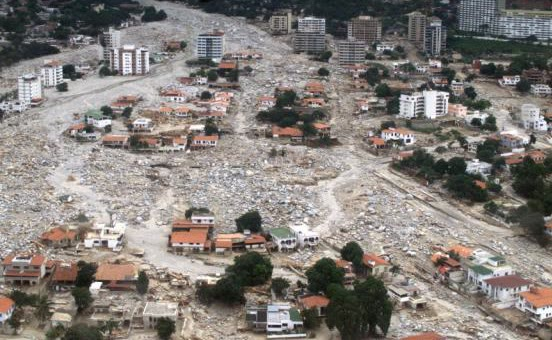
\includegraphics[width=0.62\linewidth]{images/book4/b2-28-caraballeda-debris-flow.jpg}
\par\smallskip{\small Depósitos de \omterm{def:b2:geological-hazards:slope}{fluxos de detritos} no leque de Caraballeda, no litoral da Venezuela,
depois da tempestade de dezembro de 1999: os fluxos saíram do canal principal e soterraram a cidade sob
blocos. Fotografia de Lawson Smith, U.S. Army Corps of Engineers (domínio público).}
\end{omfigure}
% ledger: photo:b2-28-caraballeda, vargas:caraballeda

\section{Os tsunamis}\label{sec:b2:geological-hazards:tsunamis}

Um tsunami produzido pelo soerguimento brusco do fundo do mar tem um comprimento de onda de dezenas a centenas de
quilômetros, muito mais que a profundidade do oceano. É uma onda longa, e sua velocidade depende apenas
da profundidade.

\begin{proposition}[Ondas longas]\label{prop:b2:geological-hazards:long-waves}
Uma onda de gravidade de superfície cujo comprimento de onda é muito maior que a profundidade $h$ da água propaga-se a
$c = \sqrt{gh}$, qualquer que seja seu comprimento de onda. Onde ela avança lentamente para águas mais rasas sem
se refletir nem quebrar, sua amplitude $A$ cresce como $h^{-1/4}$.
\end{proposition}

\begin{proof}
A relação de dispersão dá a velocidade de fase $c = \omega/k = \sqrt{(g/k)\tanh(kh)}$. Para uma onda
longa $kh = 2\pi h/\lambda \ll 1$, e $\tanh(kh) \approx kh$, logo $c = \sqrt{gh}$, independente de
$k$: as ondas longas não se dispersam. A energia da onda por unidade de área da superfície do mar é $\frac12
\rho g A^2$, e ela se propaga a $c$. Se nenhuma energia é refletida ou perdida, o fluxo $\frac12\rho g A^2
c$ através de qualquer seção é o mesmo ao longo do trajeto: $A^2 \sqrt{h}$ é constante, e $A \propto
h^{-1/4}$.
\end{proof}

Sobre \qty{4000}{m} de água um tsunami propaga-se a \qty{198}{m.s^{-1}}, \qty{713}{km/h}; sobre
\qty{5000}{m}, \qty{797}{km/h}, os ``mais de 800 km/h'' citados pelos serviços de alerta. Perto da
costa, em \qty{10}{m} de água, ele desacelera para \qty{36}{km/h}; sua frente é alcançada pela água
de trás, a onda encurta e se empina, e sua altura cresce.
% ledger: nws:tsunami-speed

\begin{definition}[Altura máxima de inundação de um tsunami]\label{def:b2:geological-hazards:tsunami}
A \emph{altura máxima de inundação de um tsunami}\index{altura máxima de inundação de um tsunami} num ponto da costa é a altura, acima do
nível do mar no momento, do terreno mais alto que a água atinge ali, terra adentro. A distância
horizontal da linha de costa até esse ponto é a distância de inundação.
\end{definition}

As equipes de levantamento medem as alturas máximas de inundação a partir de marcas de água, linhas de detritos e danos depois de cada tsunami. O
banco de dados global de tsunamis contém \num{2177} observações de altura máxima de inundação para o tsunami do oceano Índico de
26 de dezembro de 2004, produzido por um terremoto de magnitude 9.1 ao largo de Sumatra, com uma altura máxima da água de
\qty{50.9}{m}, e \num{6429} para o tsunami de 11 de março de 2011 ao largo de Honshu, também de magnitude 9.1,
com um máximo de \qty{39.3}{m}. Os dois mataram \num{227899} e \num{18423} pessoas. Em Banda Aceh,
a água atingiu o meio do segundo andar da mesquita abaixo.
% ledger: ncei:tsu-2004, ncei:tsu-2011, usgs:aceh-mosque

\begin{omfigure}
\centering
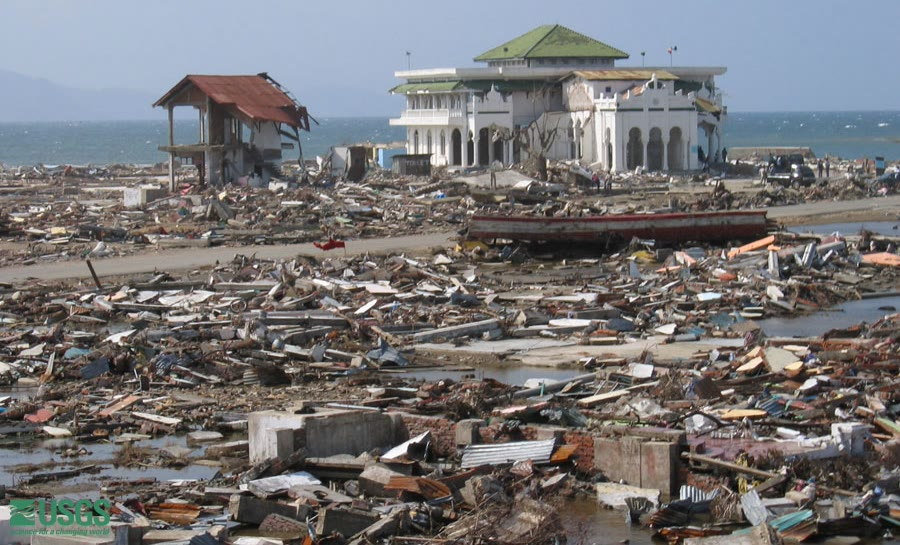
\includegraphics[width=0.62\linewidth]{images/book4/b2-28-aceh-mosque-tsunami.jpg}
\par\smallskip{\small Banda Aceh, Sumatra, em 21 de janeiro de 2005, depois do tsunami de 26 de dezembro
de 2004: uma mesquita permanece de pé no meio dos escombros dos edifícios ao seu redor. Fotografia do U.S. Geological
Survey (domínio público).}
\end{omfigure}
% ledger: photo:b2-28-aceh

\section{As cheias}\label{sec:b2:geological-hazards:floods}

\begin{definition}[Curva de frequência de cheias]\label{def:b2:geological-hazards:flood}
A \emph{curva de frequência de cheias}\index{curva de frequência de cheias} de um rio numa estação fluviométrica é a
curva da vazão de pico anual em função de seu \omterm{def:b2:geological-hazards:return}{período de retorno}, ou de sua probabilidade anual de
excedência, construída a partir do registro de picos anuais da estação e em geral estendida por uma lei de
probabilidade ajustada.
\end{definition}

A fórmula dos postos dos volumes escolares posiciona os pontos da curva. Ela tem uma razão.

\begin{proposition}[Posição de plotagem de Weibull]\label{prop:b2:geological-hazards:weibull}
Sejam $n$ picos anuais independentes e extraídos da mesma distribuição contínua, e seja
$G(x)$ a probabilidade de que o pico de um ano exceda $x$. O pico de posto $m$, contado a partir do
maior, tem uma \omterm{def:b2:geological-hazards:poisson}{probabilidade de excedência} esperada $m/(n + 1)$, de modo que é plotado em $T = (n +
1)/m$.
\end{proposition}

\begin{proof}
$U = G(X)$ é uniforme em $[0, 1]$ para uma lei contínua, e $G$ é decrescente, logo o
$m$-ésimo maior pico corresponde ao $m$-ésimo menor de $n$ variáveis uniformes independentes,
$U_{(m)}$. Sua densidade é $f(u) = \frac{n!}{(m-1)!\,(n-m)!}u^{m-1}(1-u)^{n-m}$: um dos $n$ valores
em $u$, $m - 1$ abaixo e $n - m$ acima. Com a integral Beta $\int_0^1 u^{p}(1-u)^{q}\,\mathrm{d}u
= p!\,q!/(p + q + 1)!$,
\begin{equation*}
\mathbb{E}[U_{(m)}] = \frac{n!}{(m-1)!\,(n-m)!}\cdot\frac{m!\,(n-m)!}{(n+1)!} = \frac{m}{n+1}. \qedhere
\end{equation*}
\end{proof}

O maior pico de um registro de 30 anos é portanto plotado em 31 anos, e nada no registro fixa
a cheia de 100 anos. Para alcançá-la, os picos são ajustados com uma lei de extremos, frequentemente a de Gumbel,
$\Pr(\text{pico} \leq x) = \exp\bigl(-e^{-(x - u)/\alpha}\bigr)$, cuja cheia de $T$ anos é $x_T = u
- \alpha\ln\bigl(-\ln(1 - 1/T)\bigr)$: uma reta em função de $-\ln(-\ln(1 - 1/T))$, extrapolada
além do registro com um risco que cresce com a distância.

\section{Monitoramento e alerta precoce}\label{sec:b2:geological-hazards:warning}

\begin{definition}[Sistema de alerta precoce]\label{def:b2:geological-hazards:warning}
Um \emph{sistema de alerta precoce}\index{sistema de alerta precoce} é um sistema integrado de monitoramento
de ameaças, previsão, avaliação de risco, comunicação e preparação que permite uma
ação oportuna antes de um evento perigoso. Ele reúne quatro elementos: o conhecimento do risco; a detecção,
o monitoramento e a previsão da ameaça; a difusão dos alertas; e a preparação para
responder.
\end{definition}
% ledger: undrr:ews

A física fixa quanto tempo cada alerta pode dar. As ondas sísmicas não podem ser ultrapassadas, mas as ondas S
destrutivas propagam-se a cerca de \qty{3.2}{km.s^{-1}} na crosta superior, contra \qty{5.8}{km.s^{-1}} para
as ondas P: um alerta calculado a partir das primeiras ondas P registradas perto do epicentro chega a uma cidade
antes das ondas S, em $d(1/3.2 - 1/5.8) = \qty{0.14}{s}$ por quilômetro de distância $d$, menos o
tempo de detectar e calcular. Uma cidade a \qty{100}{km} ganha no máximo \qty{14}{s}; perto da fonte uma
zona cega não ganha nada (\cref{exo:b2:geological-hazards:12}). Um tsunami que atravessa \qty{100}{km} de mar
de \qty{2000}{m} de profundidade leva 12 minutos; através de um oceano, leva horas. Em 2011, o alerta
japonês foi emitido cerca de três minutos depois do terremoto, mas com uma magnitude estimada baixa demais,
porque os instrumentos saturaram; ele foi atualizado com dados de uma boia GPS ao largo cerca de 28 minutos depois.
Registradores de pressão de oceano profundo, que convertem a pressão no fundo do mar a cada 15 segundos numa
altura da superfície do mar, transmitem hoje por satélite a passagem dos tsunamis.
% ledger: data:prem, jma:warning, ndbc:dart
% values: 0.1401 s/km, 14.0 s at 100 km; 140 m/s over 2000 m, 11.9 min per 100 km (calc/ch28.py)

\begin{inthefield}[Acompanhar uma encosta em movimento]
Numa encosta conhecida por rastejar, as equipes de monitoramento instalam instrumentos que medem as variáveis da
equação da encosta infinita. Piezômetros em furos de sondagem registram a pressão neutra na superfície de deslizamento;
tubos inclinométricos, lidos a intervalos de profundidade, mostram onde o terreno se curva e com que rapidez; estações
GNSS e extensômetros registram o movimento da superfície; um pluviômetro registra o gatilho.
As equipes comparam o movimento com a chuva e a pressão da água, estação após estação, e procuram
a aceleração que precede a ruptura.
\end{inthefield}

\section*{Exercícios}\label{sec:b2:geological-hazards:exercises}

Dados para os exercícios, salvo indicação em contrário: $g = \qty{9.81}{m.s^{-2}}$; peso específico da água
\qty{9.81}{kN.m^{-3}}; a GMPE \eqref{eq:b2:geological-hazards:gmpe} em rocha ($G_B = G_C = 0$),
$\sigma = 0.230$; velocidades P e S na crosta superior 5.8 e \qty{3.2}{km.s^{-1}}. Arredonde a três
algarismos significativos.
% ledger: bjf93:pga, data:prem

\begin{exercise}[$\star$]\label{exo:b2:geological-hazards:1}
Pelo modelo de Poisson: (a) qual é a probabilidade de pelo menos uma cheia de 100 anos em 30 anos?
(b) Qual é a probabilidade de que um século passe sem uma cheia de 100 anos? (c) Encontre o \omterm{def:b2:geological-hazards:return}{período de
retorno} do movimento com uma chance de \qty{5}{\percent} de excedência em 50 anos.
\end{exercise}

\begin{exercise}[$\star$]\label{exo:b2:geological-hazards:2}
Duas cidades enfrentam abalos fortes. Na cidade A, eles ocorrem a uma taxa de uma vez em 200 anos e
destruiriam \qty{2}{\percent} de seus 5000 edifícios; na cidade B, uma vez em 50 anos, destruindo
\qty{10}{\percent} de seus 800 edifícios. (a) Encontre o número esperado de edifícios destruídos por
ano em cada cidade. (b) Qual cidade tem o maior risco, embora tenha a menor \omterm{def:b2:geological-hazards:risk}{exposição}? (c)
Qual dos três fatores faz a diferença?
\end{exercise}

\begin{exercise}[$\star$]\label{exo:b2:geological-hazards:3}
(a) Encontre a velocidade de um tsunami sobre profundidades de 4000, 200 e \qty{10}{m}. (b) Quanto tempo ele leva
para atravessar \qty{1500}{km} de oceano de \qty{4000}{m} de profundidade? (c) A que profundidade ele se propagaria a
\qty{800}{km/h}?
\end{exercise}

\begin{exercise}[$\star$]\label{exo:b2:geological-hazards:4}
Uma areia seca e sem coesão com $\varphi' = \ang{33}$ forma uma encosta longa. (a) Encontre seu \omterm{def:b2:geological-hazards:slope}{fator de
segurança} a \ang{25}. (b) Qual é a encosta mais íngreme que ela pode formar? (c) A encosta fica saturada, com
o nível freático na superfície e percolação paralela a ela, de modo que $r_u = \gamma_w\cos^2\beta/\gamma$
com $\gamma = \qty{20}{kN.m^{-3}}$. Mostre que $F = (1 - \gamma_w/\gamma)\tan\varphi'/\tan\beta$ e
calcule-o a \ang{25}.
\end{exercise}

\begin{exercise}[$\star\star$]\label{exo:b2:geological-hazards:5}
O catálogo global contém 696 terremotos de magnitude pelo menos 7 nos 50 anos de 1976--2025, e
o intervalo médio entre eles é de 26.2 dias. (a) Encontre sua taxa anual média. (b) Pelo modelo de
Poisson, qual é a probabilidade de que 30 dias passem sem nenhum? Compare com a fração observada
de intervalos mais longos que 30 dias, 0.304. (c) Qual é a probabilidade de pelo menos um numa
semana dada?
\end{exercise}

\begin{exercise}[$\star\star$]\label{exo:b2:geological-hazards:6}
(a) Encontre a PGA mediana de um terremoto de magnitude 6.5 em rocha a $d = 0$, 10, 30 e
\qty{100}{km}. (b) Qual seria ela a \qty{10}{km} num local de classe C? (c) Entre que valores
fica a PGA em rocha a \qty{10}{km} com uma probabilidade de cerca de \qty{68}{\percent}?
\end{exercise}

\begin{exercise}[$\star\star$]\label{exo:b2:geological-hazards:7}
Os picos anuais de um rio ao longo de 12 anos foram, em \unit{m^3.s^{-1}}: 212, 148, 305, 176, 251, 133, 188,
420, 160, 229, 195, 268. (a) Dê os \omterm{def:b2:geological-hazards:return}{períodos de retorno} dos quatro maiores. (b) Estime a cheia de 10
anos interpolando linearmente em $\ln T$ entre os dois maiores. (c) Por que este registro não pode dizer
nada confiável sobre a cheia de 100 anos?
\end{exercise}

\begin{exercise}[$\star\star$]\label{exo:b2:geological-hazards:8}
Num vulcão agitado o observatório estima: agitação magmática 0.6; erupção se magmática 0.4;
explosiva se houver erupção 0.5; um \omterm{def:b2:eruptive-styles:pdc}{fluxo piroclástico} que atinge um dado vale se explosiva 0.3. (a) Encontre
a probabilidade de um \omterm{def:b2:eruptive-styles:pdc}{fluxo piroclástico} no vale. (b) Encontre a probabilidade de uma erupção, e
de uma erupção sem fluxo no vale. (c) Novos dados de deformação elevam a probabilidade de uma
erupção, se a agitação é magmática, para 0.7. Atualize (a).
\end{exercise}

\begin{exercise}[$\star\star$]\label{exo:b2:geological-hazards:9}
Um solo seco com $c' = \qty{8}{kPa}$, $\varphi' = \ang{30}$ e $\gamma = \qty{19}{kN.m^{-3}}$ repousa sobre
uma encosta de \ang{35}. (a) Encontre a espessura $z_c$ para a qual $F = 1$. (b) Encontre $F$ para uma camada
de \qty{2}{m} de espessura. (c) A mesma camada fica saturada, com o nível freático na superfície e
$r_u = \gamma_w\cos^2\beta/\gamma$. Encontre $F$.
\end{exercise}

\begin{exercise}[$\star\star\star$]\label{exo:b2:geological-hazards:10}
(a) Mostre que o modelo de Poisson não tem memória: a probabilidade de nenhum evento em $[s, s + t]$, dado
que não houve nenhum em $[0, s]$, é $e^{-t/T}$, qualquer que seja $s$. (b) Uma falha tem um \omterm{def:b2:geological-hazards:return}{período de retorno} de 475 anos para seus
grandes terremotos e não teve nenhum nos últimos 400 anos. Qual é, segundo o modelo, a probabilidade de um
nos próximos 50 anos? (c) O rebote elástico do volume do primeiro ano sugere que a probabilidade
deveria, ao contrário, crescer com o tempo desde o último terremoto. Que hipótese do modelo de Poisson
ele contradiz, e por que os mapas de ameaça mantêm o modelo para as fontes areais?
\end{exercise}

\begin{exercise}[$\star\star\star$]\label{exo:b2:geological-hazards:11}
Um tsunami de amplitude \qty{0.5}{m} e período de 20 minutos atravessa um oceano de \qty{4000}{m} de profundidade. (a)
Usando o argumento do fluxo de energia da proposição sobre as ondas longas, encontre sua amplitude em \qty{10}{m}
de água. (b) Encontre seu comprimento de onda nas duas profundidades. (c) Dê duas razões pelas quais a altura máxima de inundação na costa
pode diferir muito desta estimativa.
\end{exercise}

\begin{exercise}[$\star\star\star$]\label{exo:b2:geological-hazards:12}
Um \omterm{def:b2:geological-hazards:warning}{sistema de alerta sísmico precoce} emite um alerta 4 segundos depois que a onda P atinge sua estação
mais próxima do epicentro, a \qty{10}{km}. Despreze a profundidade da fonte. (a) Quando o
alerta é emitido depois do terremoto? (b) Quantos segundos antes da onda S uma cidade a \qty{50}{km}
do epicentro o recebe? E uma cidade a \qty{100}{km}? (c) Encontre o raio da zona cega, onde
a onda S chega antes do alerta.
\end{exercise}

\begin{problem}[{Problema de fim de semana --- uma cidade entre uma falha e uma encosta}]\label{pb:b2:geological-hazards:1}
Uma cidade sobre rocha fica a \qty{10}{km} de uma zona sismogênica; todos os seus terremotos são tomados a
$d = \qty{10}{km}$. Sua recorrência é $\log_{10} N(\geq M) = 4.0 - 1.0\,M$ por ano para $M \geq 5$,
truncada em $M_{\max} = 7.5$. O abalo segue a GMPE \eqref{eq:b2:geological-hazards:gmpe}
com $\sigma = 0.230$. Acima da cidade, uma camada de solo de \qty{3}{m} de espessura repousa sobre uma encosta de \ang{30},
com $\gamma = \qty{19}{kN.m^{-3}}$, $c' = \qty{4}{kPa}$ e $\varphi' = \ang{34}$; a água tem peso
específico \qty{9.81}{kN.m^{-3}}. Arredonde a três algarismos significativos.

\noindent\textbf{Parte I --- Recorrência.}
\begin{enumerate}
  \item Encontre as taxas anuais de terremotos de magnitude pelo menos 5, 6 e 7, ignorando a
        truncagem.
  \item Dê os \omterm{def:b2:geological-hazards:return}{períodos de retorno} correspondentes.
  \item Com a truncagem, encontre a taxa de terremotos acima de 7.5, e a taxa dos que ficam entre 7
        e 7.5.
  \item Encontre as taxas das classes de magnitude 5--6 e 6--7.
  \item Qual é a probabilidade de pelo menos um terremoto de magnitude 6 ou mais em 50 anos?
  \item E de magnitude 7 ou mais?
\end{enumerate}

\noindent\textbf{Parte II --- O movimento do solo na cidade.}
\begin{enumerate}[resume]
  \item Encontre $r$, e o termo de distância $-0.778\log_{10} r$.
  \item Represente as três classes pelas magnitudes 5.5, 6.5 e 7.25. Encontre o
        $\log_{10}\mathrm{PGA}$ mediano e a PGA mediana de cada uma.
  \item Encontre a PGA excedida com uma probabilidade de \qty{16}{\percent} por uma magnitude 6.5.
  \item Qual é a probabilidade de que uma magnitude 6.5 produza mais de \qty{0.3}{g}?
  \item Qual é a PGA mediana do maior terremoto possível?
\end{enumerate}

\noindent\textbf{Parte III --- A curva de ameaça.}
\begin{enumerate}[resume]
  \item Encontre a taxa anual de excedência de \qty{0.2}{g}, somada sobre as três classes.
  \item O mesmo para \qty{0.3}{g}.
  \item O mesmo para \qty{0.4}{g}.
  \item Que taxa anual corresponde a \qty{10}{\percent} em 50 anos?
  \item Entre quais dos três níveis fica essa taxa?
  \item Interpolando linearmente em $\ln\lambda$ em função de $\ln a$, encontre a PGA com uma
        chance de \qty{10}{\percent} de excedência em 50 anos.
  \item Que classes contribuem mais para a taxa a \qty{0.3}{g}? Comente, usando a resposta à
        questão~11.
\end{enumerate}

\noindent\textbf{Parte IV --- A encosta acima da cidade.}
\begin{enumerate}[resume]
  \item Encontre o \omterm{def:b2:geological-hazards:slope}{fator de segurança} da encosta seca.
  \item Encontre-o quando a camada está saturada, com o nível freático na superfície ($r_u =
        \gamma_w\cos^2\beta/\gamma$).
  \item Até que fração da espessura da camada o nível freático pode subir antes que a encosta rompa?
  \item Numa análise pseudoestática (admitida), o abalo acrescenta uma força horizontal $kW$. Encontre o
        $k$ crítico da encosta seca, para o qual $F = 1$.
  \item Tomando $k$ igual à PGA em unidades de $g$, que magnitude produz o valor crítico como
        sua mediana na cidade? Compare com a resposta à questão~17.
  \item Em resumo: qual é a \omterm{def:b2:geological-hazards:psha}{aceleração de pico do solo} com uma chance de \qty{10}{\percent} de ser
        excedida em 50 anos na cidade?
\end{enumerate}
\end{problem}
